\cleardoublepage
\chapter{Design and Specialisation}\label{sec:contrib1}\minitoc\vspace{.5cm}
\index{Contribution 1}

\section{Introduction}
\sidenote{Overview}
As outlined in the introduction, the goal of this thesis is to design and implement a semantic annotation extension of the OpenMTC Platform aiming to provide semantic interoperability for accessing resources and interpreting data from different stakeholders. This goal is a part of the overall goal of the IIoT department which aims at moving the OpenMTC platform towards an intelligent Fog Node framework (OpenIoTFog).
This extension allows OpenMTC to create a pool of common data available in a specific environment and to share them between different OpenMTC applications, without requiring the information of the data type or content (units, metadata, context, etc.) in advance. Moreover, our implementation consist as well in enabling data access via SPARQL interface and OneM2M standard. The figure .1.1 demonstrate an overall picture of the whole concept.\par


\section{Overall Architecture}

The high-level functional architecture specified by oneM2M is adapted to define the detailed architecture of the semantic annotation extension. In this context, M2M middleware platforms provide huge advantages when it comes to Smart City implementations. Hence, it is expected to provide interoperability and communication between machines “things” and their virtual representation on the M2M middleware to support object addressing, tracking, and discovery as well as information representation, storage, and exchange. In this section, we specify a semantic annotation extension aiming to provide semantic interoperability within an M2M system. Figure 5.2 depicts the High-level architecture of the semantic annotation extension within an M2M service middleware. In such a oneM2M compatible system the semantic annotation extension is considered to be located in the frontend as well as the backend of the system. \par
The M2M middleware aligned with oneM2M standard specification compromise three different functions as depicts in the figure. The first function is the Application Entity (AE) which implements an M2M application service logic as specified in []. Each instance executed by an application service logic is named “Application entity” (AE) that can be resident in some M2M nodes and more than once on a single M2M node. The second function is Common Services Entity (CSE) which represents an instantiation of common service functions of the M2M environments. It offers several different service functions such as Data Management, Device Management, Subscription Management, and Location Services. The last function is the Network Services Entity (NSE) which provides services from different networks to the CSEs. In the context of the roles of Mca interface, it provides communication between different oneM2M CSEs. A description of the implemented capabilities within the prototype system is given in the next chapter. 
\par
\begin{figure}[htbp]
    \centering
    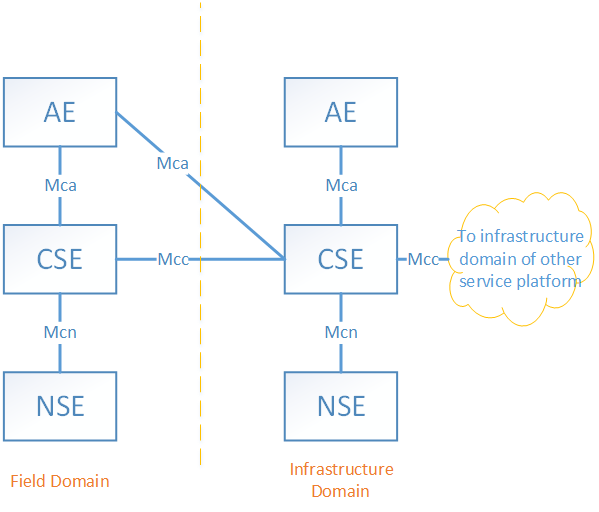
\includegraphics[width=.9\textwidth]{resources/images/arch}
    \caption{oneM2M Functional Architecture}\label{fig:contrib1:goal}
\end{figure}\par
There are a huge number of connected M2M and non-M2M devices within an M2M network. Therefore our semantic annotation extension considers different architecture designs to deal with this heterogeneous devices. Since that, most of the devices connected to the M2M network are more likely to face energy shortages, and they are often presented with limited storage capabilities, they can't interact immediately to all transaction with each other or with another component in the network, this situation will cause cancellation of the transaction and many other problems. Therefore, REST based architecture is considered within the semantic annotation extension as well as any M2M system. In fact, REST is based on the concept of resource addressed by URLs. Thus it provides to the different devices connected to the M2M network a way to store their states and data. In this manner, our semantic annotation extension makes use of the internal subscription/notification mechanism provided by the inner-API which is mainly based on events to subscribe in oneM2M system to a targeted resources. The CSE sends back notification as soon as the data is available or updated which enables the extension to get used to the targeted data. Figure illustrate the M2M resource tree evaluated in our extension.  In this context, each device in the M2M system is presented by a uniquely addressable resource in the hierarchical tree. For example, a device can be presented by a <device\textunderscore name> resource under the hosting getaway resource <scl>. Application in the other hand is presented by <application> resource that includes one or more resource type container to classify different <contentInstences> resources under it, where the targeted data are generally located.\par
\begin{figure}[htbp]
    \centering
    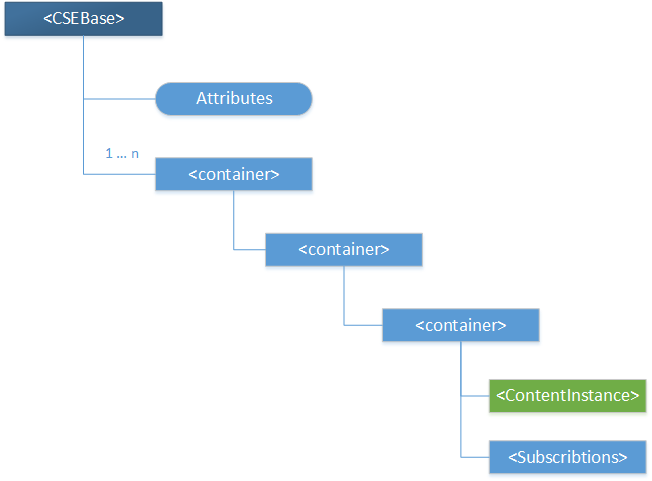
\includegraphics[width=1\textwidth]{resources/images/tree}
    \caption{M2M Resource Tree based on ETSI/oneM2M specifications}\label{fig:contrib1:goal}
\end{figure}
Moreover, since our semantic annotation extension is mainly dealing with sensor data, it adapt the publish/subscribe architecture as well, which facilitate the exchange between sensor networks and cloud-based networks. The publish/subscribe architecture presents a dynamic network pattern to deliver sensor driven processed data to subscriber. It also create a decoupling communication between publisher and subscriber based on time, space and control flow. (Add Request Routing)\par
In most of the cases, those devices and sensors are a non-M2M devices which generate a huge amount of data that need to be semantically annotated and exchanged. To deal with such an issue, the semantic annotation extension consider the interworking proxy entity (IPE) which is a specialized AE defined by oneM2M for interworking with non-oneM2M system as showing in the figure. IPE includes two main functionalities:  
\begin{itemize}
\item translate a non-M2M interface non-oneM2M protocols and massages to oneM2M ones via the Mca interface
\item Mapping non-oneM2M data models into oneM2M resources, which are eventually exposed to oneM2M services.
\end{itemize}\par
Adapting this approach within the core design of our work provide a unique solution that enables communications between different protocols and most importantly, it enables semantic information exchange as well as data sharing [] among the different deployments.


\section{Detailed design model}

\subsection{Overview}
As mentioned in the previous section the design architecture of our work is composed mainly of 4 principle modules. Each module is located in a specific area within the M2M system. The detailed design model of each module is presented in the next subsections.
\sidenote{Intro}


\sidenote{Goal}

\sidenote{Approach}


\subsection{Design and specification of the semantic annotator}

\sidenote{Overview}
The semantic annotator is the most important component of our work as it is responsible for semantically annotating sensors, devices and the type of information they produce (e.g., context of the data, units of the data, type of the data, the location/address, etc.). Hence, the network applications will have the possibility to discover, share and understand the information from different device applications. The main idea of the semantic annotator is to create a child resources for the targeted resources to help represent semantic information. As presented in the previous section, a “resource” is a resource that is addressable using a uniform resource identifier (URI) and stored in the resource repository of a given M2M system, such as the resource tree in oneM2M as shown in the figure (e.g. AE, container, contentlnstance, etc.). In addition, a resource is a uniquely addressable entity in the RESTful oneM2M architecture. It is possible to transfer and manipulate the resource representation by using the four major RESTful methods such as Create, Retrieve, Update, and Delete (CRUD). Moreover, each resource may contain one or more child resources and attributes that store a different set of information about the resources. A child resource is a resource that has a containment relationship with a parent resource. Each child resource is referenced within the representation of its parent resource. Thus, the lifetime of each child resource is limited to its parent’s resource lifetime.\par
Table highlight examples of resources and related child resources defined by TS-0001- OneM2M Functional Architecture version 3. 


\sidenote{Approach}
The M2M architecture provides procedures to discover the different resources available in a specific CSE within a given M2M system. This procedure is knowing as the resource discovery procedure (TS-0018). It is mainly processed using the RETRIEVE method which retrieves the information presented or stored in the resource’s attributes. This can be done by sending a request from a specific originator (e.g. CSE or AE) to a given receiver by including the name of the target attribute in the Content parameter in the request message. When receiving the request, the receiver verifies the presence of the requested resource and checks the originator privileges for retrieving the information related to the resource. The Receiver returns the requested information only if the verification is successfully done. Otherwise, an error is returned instead. Figure TS-0018 present the mentioned procedure for retrieving a given resource.\par
Moreover, as specified in oneM2M-TS-0001 oneM2M Functional Architecture version 3, the usage of the resource discovery procedures can be customized with specified Filter Criteria parameter which limits the scope of the results. To be more specific, the filter criteria parameter provides rules description for resource discovery, (e.g. creation time, resource types, etc.).\par
Using the conventional M2M service layer mechanisms together with the filter criteria can provide effective resource discovery, however, it is not as advanced as we expect for querying resources. Therefore, our semantic annotator’s design consist of providing more advanced mechanisms in order to achieve a more advanced resource query execution. The main design architecture of the semantic annotator aims at realizing semantic-based query by annotating the target resources semantically. In the context of this disclosure, the semantic annotator aims at creating and adding as a child resource the semantic representation of the parent resource. In this manner, all the targeted resources provide a specific semantic representation which allows more advanced query based on semantic.\par
As defined in OneM2M functional Architecture, the type of the resources aiming at providing a semantic representation of target resources which are created by our semantic annotator, is <semanticDescriptor> which will be discussed in more details herein. This type of resources is a crucial component of the semantic annotator design as it allows the storage of the semantic information which principally includes relationship and value information of a given resource in its child resource. Storing the different semantic information in the <semanticDescriptor> resources allows the extraction and the storage of this information in a semantic repository. The semantic repository presented in the next subsection contains mainly a set of triples allowing semantic-based query execution. Also, each semantic annotation instance includes an identifier which is defined by the resource type <semanticDescriptor> associated with some random donation (e.g., a code that may be alphabetic). The main architecture of the semantic annotator instance or the resource type <semanticDescriptor> consist of associating this type of resources with the resources that is included in it's tripled. Thus, each resource type < semanticDescriptor> is mapped to the URIs of the resources of resource repository stored in hierarchical M2M resource structure.  The figure illustrate the M2M Resource Tree that includes the resource type < semanticDescriptor>.\par
\begin{figure}[htbp]
    \centering
    \includegraphics[width=.8\textwidth]{resources/images/resources}
    \caption{M2M Resource Tree based including resource type < semanticDescriptor> }\label{fig:contrib1:goal}
\end{figure}

\sidenote{Integration}
As discussed previously the resource type semantic descriptor is a key of importance for supporting semantic interoperability within an M2M system or M2M service middleware that adapt the oneM2M architecture. This can be done by storing the different semantic descriptions of the targeted resources in its child resources. Within our work, the semantic description is mainly provided by different ontologies which will be discussed in more details in the next subsection. As a result, a targeted resource can have multiple semantic description resources as child resources in case it is semantically described by more than one ontology as showing in the figure bellow.  \par
According to the ETSI/oneM2M specification, each resource in the M2M system includes one or more attribute. This attributes comprises information pertaining to the resource. Moreover, each attribute has a unique name that belongs only to a given resource and value. The resources attribute are uniquely addressable as well. In the table, a set of common attributes of M2M resources is presented.
In the M2M architecture, those attributes are commonly used by all announced resources including the resource type semantic descriptor. Besides the common attributes, there are more specific attributes for the semantic descriptor. Those attributes are shared by all announced < semanticDescriptor > specializations.\par
As specified in oneM2M TS-0004 Service Layer Core Protocol Version 2.7.1, semantic descriptor resource includes five mandatory and optional attributes as showing in the figure.
\begin{figure}[htbp]
    \centering
    \includegraphics[width=1\textwidth]{resources/images/strc}
    \caption{Structure of < semanticDescriptor> resource }\label{fig:contrib1:goal}
\end{figure}
\subsubsection{Mandatory attributes}
Mandatory attributes mean that in case one of this attributes is missing while creating the resource type semantic descriptor, an error would be throwing back, and the creation of the resource is abandoned.
Those attributes are: 

\paragraph*{Descriptor attribute:}

Each semantic descriptor must provide exactly one descriptor attribute. This attribute is responsible for storing the semantic description of the resource whose child resource the <semanticDescriptor> resource is. As mentioned previously, a semantic description is mainly provided by different ontologies within the semantic annotator architecture. More specifically this description shall be according to subject-predicate-object triples as defined in the RDF graph-based data model [4]. The encoding of the RDF triples used in oneM2M is xs:base64Binary as defined in oneM2M TS-0004 Service Layer Core Protocol Version 2.7.1[TS-0004]. Base64Binary is a representation of arbitrary Base64 encoded binary data. To be more specific data in the base64Binary format are encoded using Base64 encoding defined in RFC 4648 [9], which is derived from in RFC 2045 [10].
\paragraph*{RelatedSemantics attribute:}

For creating a new semantic descriptor resource about a resource and potentially subresource within the semantic annotator design, the semantic descriptor resource must contain exactly one related Semantic attribute. As indicated in its name this attribute provide a list of URIs for resources containing related semantic information to the resources where it was created. The URI(s) aims at referencing other <semanticDescriptor> resources. This attribute is importance because it provides means to execute SPARQL queries. This attribute will be presented and explained in more detail in the data access section.
\paragraph*{DescriptorRepresentation attribute:}

Each semantic descriptor must provide exactly one DescriptorRepresentation attribute. This attribute specifies the serialization type of the descriptor attribute. It has a fixed value “application/rdf+xml:1”  which consist of a string composed of a media type followed by an “m2m: encoding” separated by “:” character. 
\subsubsection{Optional attributes}
As defined in oneM2M TS-0004 Service Layer Core Protocol Version 2.7.1[TS-0004], resource of type <semanticDescriptor> can have one or more optional attribute that provide further information depending on the M2M system.
\paragraph*{SemanticOpExec attribute:}
The semanticOpExec attribute contains a SPARQL update request which aims at updating the descriptor attribute. Thus, it is not created or retrieved. 
\paragraph*{OntologyRef attribute:}
 The ontologyRef attribute provide a reference URL of the ontology used to semantically describe the information that is stored in the descriptor attribute. Hence, it is highly recommended to use this attribute in case the information can be described using more than one ontology.\par
The table below summarize all the specific attributes of the semantic descriptor resource.

\begin{landscape}
   \begin{table}[]
\centering
\caption{Attributes of the semantic descriptor resource}
\label{my-label}
\begin{tabular}{llllll}
\hline
\textbf{<SemanticDescriptor> attributes}                              & \textbf{Role}                                                                                                                                                                      & \textbf{Data type}                                                                  & \textbf{Default value}                                                    & \textbf{Mandatory}             & \textbf{Optional}              \\ \hline
\textbf{descriptorRepresentation} & \begin{tabular}[c]{@{}l@{}}specify the serialization \\ type of the descriptor\\ attribute\end{tabular}                                                                   & \begin{tabular}[c]{@{}l@{}}Semantic content \\ representation\end{tabular} & \begin{tabular}[c]{@{}l@{}}application/\\ rdf+xml:1\end{tabular} & \multicolumn{1}{c}{X} &                       \\\midrule
\textbf{semanticOpExec}           & \begin{tabular}[c]{@{}l@{}}Update the descriptor \\ attribute\end{tabular}                                                                                                & SAPRQL                                                                     &                                                                  &                       & \multicolumn{1}{c}{X} \\\midrule
\textbf{descriptor}               & \begin{tabular}[c]{@{}l@{}}Storing the semantic \\ description of the targeted\\ resource\end{tabular}                                                                    & \begin{tabular}[c]{@{}l@{}}base64Binary \\ encoded data\end{tabular}       &                                                                  & \multicolumn{1}{c}{X} &                       \\\midrule
\textbf{ontologyRef}              & \begin{tabular}[c]{@{}l@{}}Provide a reference URL \\ of the ontology used to\\ semantically \\ describe the information \\ in the descriptor attribute\end{tabular}      & URL                                                                        &                                                                  &                       & \multicolumn{1}{c}{X} \\\midrule
\textbf{relatedSemantics}         & \begin{tabular}[c]{@{}l@{}}Provide a list of URIs \\ for resources containing\\ related semantic \\ information to the\\  resources where \\ it was created.\end{tabular} & List of URL                                                                &                                                                  & \multicolumn{1}{c}{X} &                       \\ \hline
\end{tabular}
\end{table}
\end{landscape}
\subsubsection{OneM2M procedures on SemanticDescriptor resource}

As discussed in the last section, each entity in an M2M system that follows the oneM2M architecture is represented as a uniquely addressable resource (e.g. CSE or AE). Thus it is possible to process modify and retrieve resources in oneM2M system. This section specifies the different procedures involved to manipulate information pertaining to a resource of type <semanticDescriptor> and which are located in a standardized resource structure.\par

The information exchange within a procedure is based on the use of Request/Response messages between an originator and a receiver. For example a request/response communication between different CSEs through the Mcc reference point or between AEs and a CSEs through the Mca reference point. The figure illustrates the general flow between an originator and a receiver.\par
\begin{figure}[htbp]
    \centering
    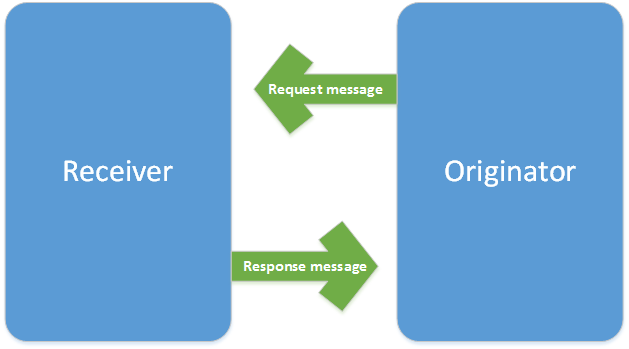
\includegraphics[width=.6\textwidth]{resources/images/response-request}
    \caption{General Flow }\label{fig:contrib1:goal}
\end{figure}
The originator sends a request message over the Mca and Mcc reference points that includes mandatory and optional parameters. The principle mandatory parameter includes mainly the address of the targeted resources, the identifier of the originator and finally the operation to be executed on the resource such as Create, Retrieve, Update, or Delete (CRUD). In case the originator possesses all the privilege to access the resource requested, the receiver send a response message back over the Mca and Mcc reference points. The response message contains mainly mandatory parameters, but it may contain optional parameter as well. The type of parameters returned in the response depends upon the requested operation (CRUD) or the mandatory response code. Therefore, this clause aims at describing the resource type <semanticDescriptor> specific primitive behavior for CRUD operations to communicate efficiently with oneM2M compliant M2M Platform System.\par

\subsubsection*{General resource request procedure for originator }

The Originator shall go through the following action in order to execute a CRUD (in this case a create request) request on a targeted CSE or AE.\par
\begin{figure}[htbp]
    \centering
    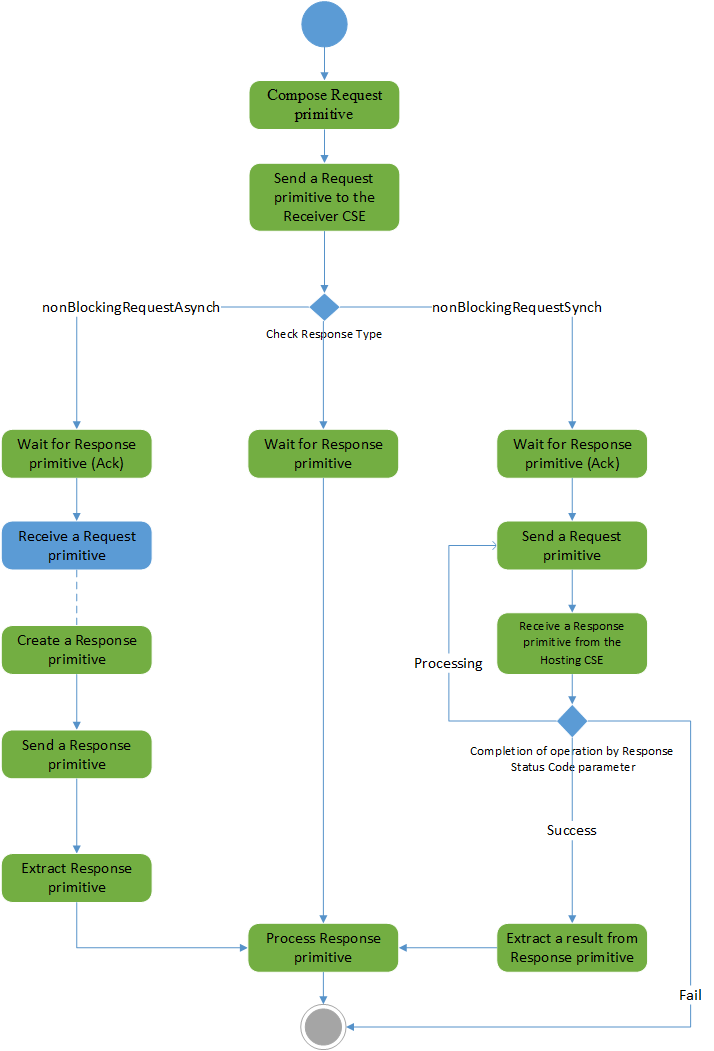
\includegraphics[width=1\textwidth]{resources/images/ori}
    \caption{General procedure of Originator }\label{fig:contrib1:dia}
\end{figure}
As showing in the diagram in Figure~\ref{fig:contrib1:dia}, the first step that should be done by the originator is to compose request primitive message which is mapped to a specific protocol. It is necessary to include in the request message the mandatory parameters previously mentioned such as the operation type, the address of the targeted resources and the identifier of the originator.\par
The second step consists of sending the request message previously composed to the desired CSE. Therefore the originator needs to determine the receiver CSE before sending. 
In the third step, the originator checks if the Response Type parameter is included in the response message. In case it exist, the originator determines the communication method from the Response Type parameter otherwise as specified in oneM2M TS-0004 Service Layer Core Protocol the communication method is set as “blockingRequest” which means that the Receiver CSE responds with the result of the requested operation after finishing processing it. The Response Type parameter includes mainly two different communication method:
\begin{itemize}
\item \textbf{nonBlockingRequestSynch:} based on Onem2M functional architecture, this kind of communication method means that in case the request is accepted by the Receiver CSE, the Receiver CSE responds, after acceptance, with an Acknowledgment confirming that the Receiver CSE will further process the request. As showing in the diagram, several steps follow this Response Type. As specified in the OneM2M functional architecture, within the first step the originator waits for a response from the receiver that corresponds to the sent request. The second step consists of sending a request primitive message from originator to the receiver. The originator must include in the request the mandatory parameters previously mentioned and optionally the optional parameter.  After successfully delivering a request primitive message to the hosting CSE, the originator shall receive mandatory parameters such as the Response Status Code, Request Identifier, and Content. The next following steps depend on form the Response Status Code. If the Response Status Code is successful (e.g. 2000, 2001, 2002, or 2004) and Content parameter exists, the result is extracted from the Response primitive and as a final step the originator process the response. Otherwise, if the Response Status Code is acknowledgment which indicates processing at the Receiver, the originators shall send a new Request primitive message. Finally, in case the Response Status Code is an error (e.g. 4XXX, 5XXX or 6XXX) or the Content parameter does not exist, it moves to finish with an error.
\item \textbf{nonBlockingRequestAsynch:} without going into the details, this method is the same as nonBlockingRequestSynch except that the result of the requested operation is sent back as a notification(s) to the notification target(s).  Therefore, as showing in the diagram, the request procedure compromise additional steps. As specified in the OneM2M functional architecture, within the first step the originator receives Request primitive with mandatory parameters such as operation, Content. In this case, the Operation parameter shall be Notify, and the Content includes notification information related to the originator.  After receiving the Request primitive, the originator shall compose a Response primitive including the mandatory parameters which are Response Status Code and Request Identifier and then send it. After sending the response to the receiver the originator extract the result from the response primitive previously received.
\end{itemize}
\subsubsection*{General request procedure for receiver }

Several steps should be executed by the receiver in a specific order to process a request received from an originator. The receiver shall execute and send an error response in case any error appears in the steps demonstrated in the diagram in Figure~\ref{fig:contrib1:reci}.\par
\begin{figure}[htbp]
    \centering
    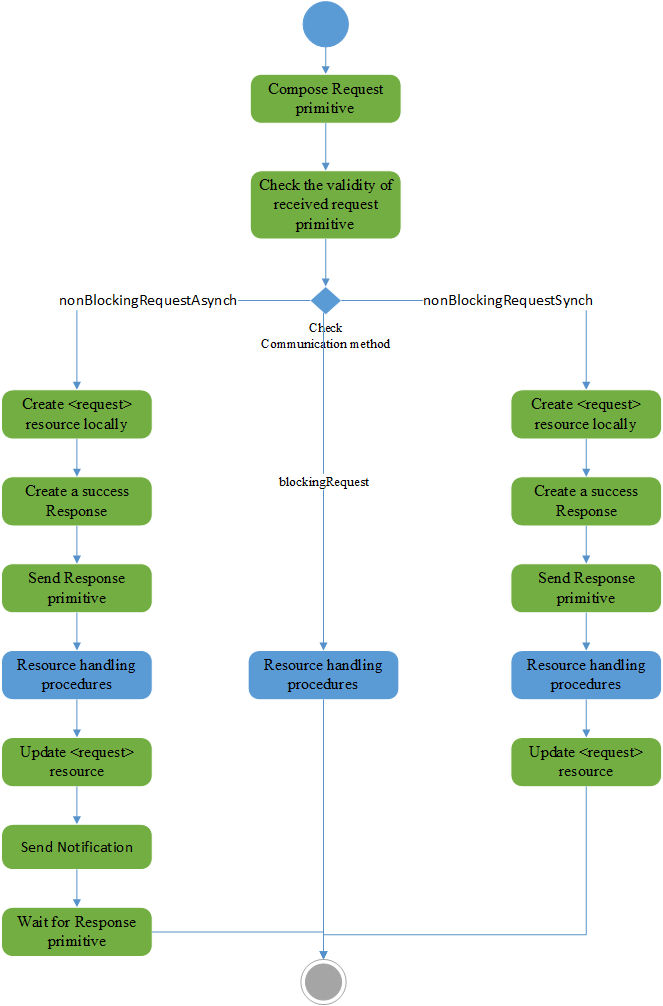
\includegraphics[width=1\textwidth]{resources/images/reci}
    \caption{General procedure of receiver }\label{fig:contrib1:reci}
\end{figure}
Based on the oneM2M specification [ts004], the first step consists of validating the received resource representation against the provided schema definitions.\par
The next step for the receiver CSE is to check the request method received by using Response Type parameter. In case the request is blockingRequest, or the Response Type is not included, it moves to the resource handler procedure step. This step will be discussed in more details herein. Otherwise, if the request is nonBlockingSynch, the receiver CSE shall create <request> resource locally which provide full support for a standardized interface to information representing the context and current status of a request [ts001]. Then the hosting CSE shall create a success response primitive including a response statute code such as CREATED for Create operation, Ok in the case of Retrieve operation, UPDATED for Update operation or DELETED in the case of Delete operation and then send it or forward it back to the originator. After sending the response primitive message, the Receiver goes to the resource handler procedure step which will be presented herein. As a final step, the hosting CSE shall update the <request> resource previously created.
In the case of a nonBlockingAsynch request, the receiver goes through the same steps previously discusses with two extra steps. When the requested operation for a nonBlockingAsynch request is completed, the hosting CSE of the resource shall send a Notify request primitive to inform the final result of requested operation against the oneM2M resource [ts004]. Finally, the originator shall wait for the Response primitive message from the receiver that corresponds to the Request primitive that was previously sent.\par
The receiver goes through a common step in all the different Response type received. The resource handler procedure step. This step calls for extra steps specified for each CRUD operation.
\begin{figure}[htbp]
    \centering
    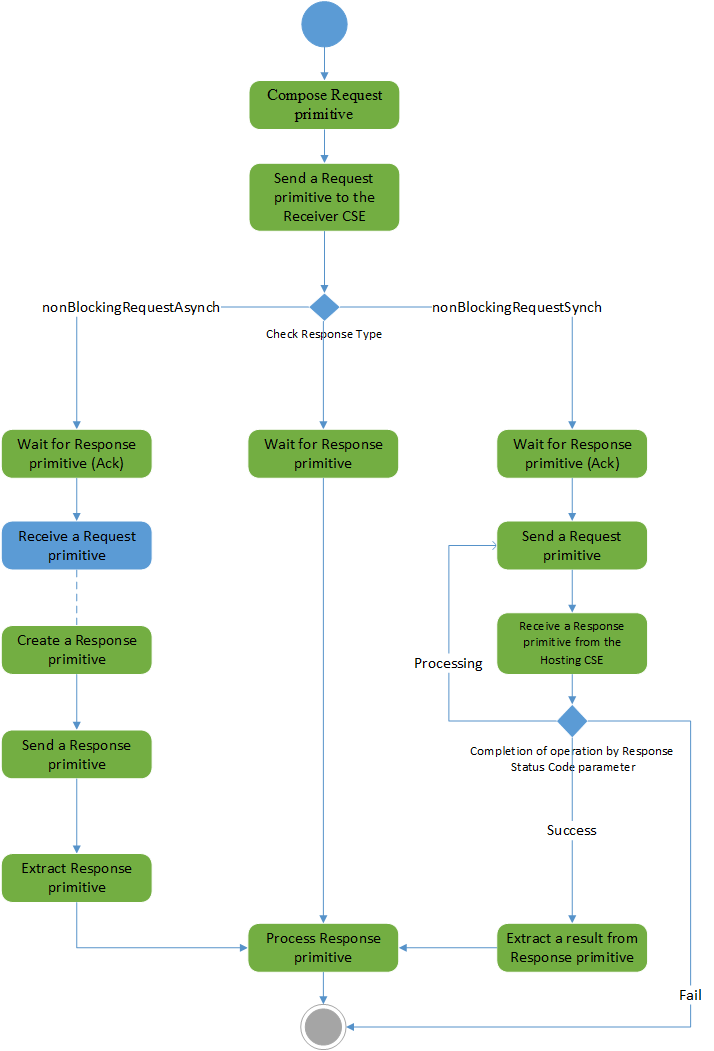
\includegraphics[width=1\textwidth]{resources/images/resource}
    \caption{General procedure of resource handling procedure }\label{fig:contrib1:re}
\end{figure}
 The figure depicts the general procedure to resource handling procedure.\par
The figure bellow describes <semanticDescriptor> resource specific primitive behavior for all CRUD operations for the receiver that specifies the resource handling procedures. \par
The first step is to check whether the receiver is Registrar CSE, the Originator is AE, and operation is created. If the receiver is Registrar CSE and Originator is an AE, the receiver shall check if the sender is allowed to create resource type specified in resource type parameter. Otherwise, check if the receiver is a hosting CSE of the incoming request or a transit CSE. In case the receiver is the hosting CSE, the receiver shall verify the existence of the addressed resources then depending on the target resource type, the Hosting CSE shall check the access control rules of the originator. If there is any rule satisfying all the specific conditions, then the evaluation is successful. Otherwise, it is failed. In the case of success, the receiver shall at first check the validity of resource representation for the CRUD operation requested. For Create and Update CRUD operation there are several extra steps to go through which will be discussed herein.\par
In the case of a valid resource representation, the specific CRUD operation is performed which consist of Creating, Retrieving, Updating or Deleting the resource. The next step consists of announcing the resources in case it contains a specific attribute named “announceTo.” As defined in TS001 an announced resource is a resource at a remote CSE that is linked to the original resource that has been announced, and it maintains some of the characteristics of the original resource. After verifying whether the resource is anounceble or not, the receiver CSE checks the communication method. As mentioned previously in this clause there are three methods of communication. If the request was blockingRequest or Response Type parameter was not included, the receiver composes a success response. Otherwise, it moves to finish. As a final step if the receiver is Hosting CSE, the overall procedure comes to an end by sending the response primitive. In case the receiver is a transit CSE, it needs to execute a Communication Management and Delivery Handling (CMDH) message forwarding procedure only if the Receiver supports the CMDH processing. As defined in ts004, if the Receiver is not compatible with CMDH processing, it shall carry out message forwarding.\item
Depending on the CRUD operation the resource request procedure for the originator and/or the receiver differ slightly from the general procedure previously discussed.\par
\subsubsection*{Create Operation }

For the Create operation, the resource request procedure for the originator keeps the same structure as the general procedure.
In the other hand, when processing the request by the receiver, the descriptor attribute should be a valid RDF/XML syntax. Therefore there are several steps to validate the resource representation before performing the Create Operation. Those specific actions are presented in the diagram in figure \ref{fig:contrib1:create} 
\begin{figure}[htbp]
    \centering
    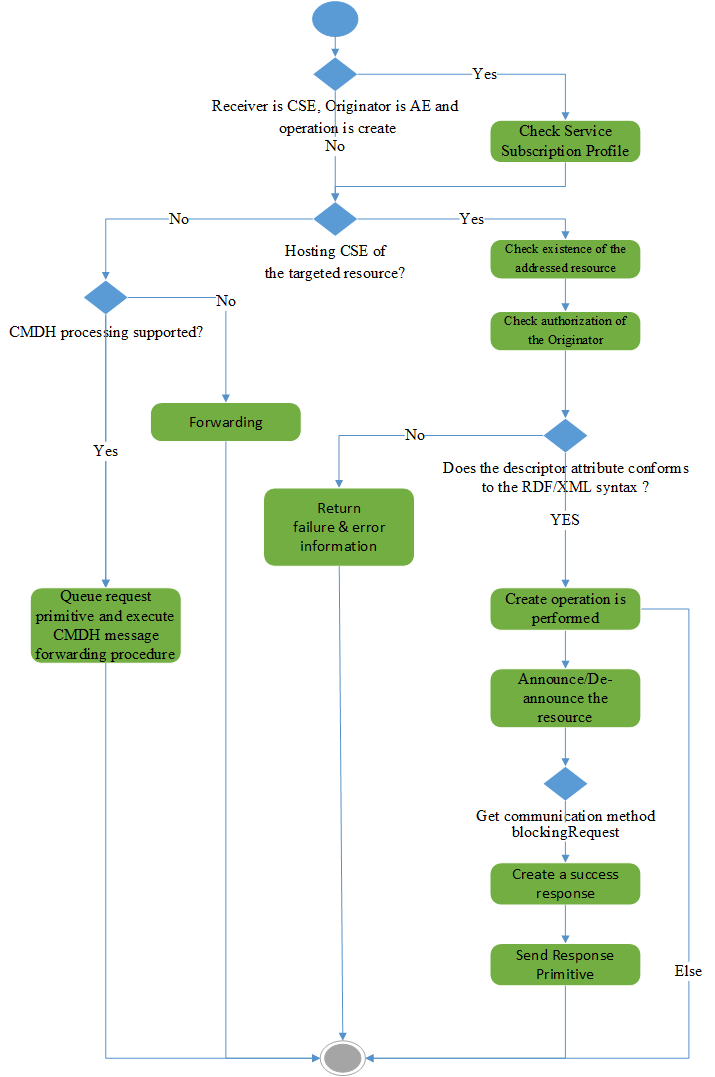
\includegraphics[width=1\textwidth]{resources/images/create}
    \caption{General procedure of Create Operation for the receiver }\label{fig:contrib1:create}
\end{figure}
There is mainly one decision to deal with. In case the descriptor attribute is not a valid RDF/XML syntax as defined in RDF 1.1 XML Syntax, the Hosting CSE return failure, and error information as a response to a CRUD operation format.
\subsubsection*{Retrieve Operation}
The Retrieve operation remains the general resource request procedure for both originator and receiver except that the response message never includes the semanticOpExec attribute.
\subsubsection*{Update Operation}
There is mainly two methods used to update the descriptor attribute:
\begin{itemize}
\item By using the standard method specified in OneM2M architecture to change the descriptor attribute with the new RDF/XML information.
\item By using a SPARQL update by composing a request to update the semanticOpExec attribute in which the value is set to an SPARQL request with SELECT or DELETE statement as specified in the SPARQL query language[]. Thus, the Update operation for the originator keeps the same structure of the general resource request procedure with customizing the "Compose Request primitive" procedure to update the semanticOpExec attribute as mentioned previously.
Concerning the Receiver, when processing the request received, two steps should be modified. 
\end{itemize}
The modification is illustrated in the diagram of the figure \ref{fig:contrib1:update}.
\begin{figure}[htbp]
    \centering
    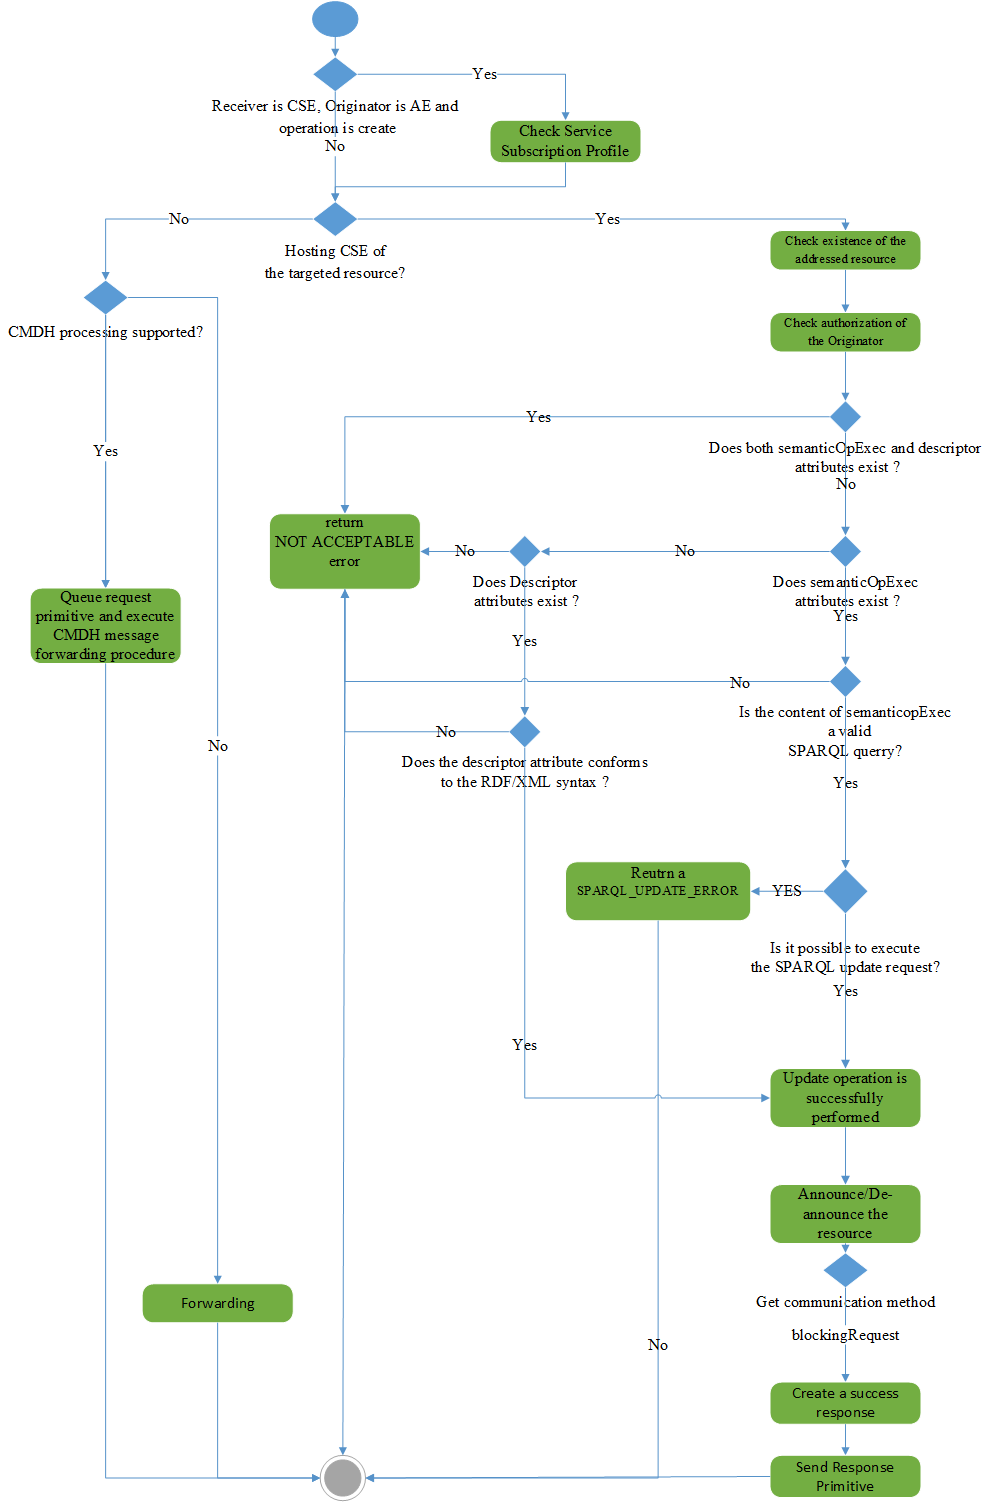
\includegraphics[width=1.1\textwidth]{resources/images/update2}
    \caption{General procedure of Update Operation for the receiver }\label{fig:contrib1:update}
\end{figure}
 First, the "Check validity of resource representation" step need to be modified as follow. The receiver shall check whether both, the semanticOpExec and descriptor attribute exist. If both exist, then the Hosting CSE shall return "NOT\textunderscore ACCEPTABLE" error as specified in OneM2M TS004. Otherwise, if the semanticOpExec only exist, the hosting CSE shall verify if the value of the attribute conforms to a valid SPARQL request. In case it does not conform to a valid SPARQL request, it shall return an "NOT\textunderscore ACCEPTABLE" error. In case the descriptor attribute exist, the receiver shall check if the new information provided conforms to the RDF/XML syntax. Otherwise, it shall return an "NOT\textunderscore ACCEPTABLE" error as well. \item
In the "Update operation is performed" step, if the semanticOpExec attribute exists, the hosting CSE shall execute the SPARQL request. In the case of failure, the receiver shall return "SPARQL\textunderscore UPDATE\textunderscore ERROR" error. Otherwise, it goes to the next step which was previously explained.
\subsubsection*{Delete Operation}
The procedure of Delete operation reminds the same as the general procedure for both originator and receiver.


\subsection{Design and specification of the Semantic Repository}
\subsubsection{Introduction}
\sidenote{Overview}
The preceding subsection described the detailed architecture of the semantic annotator responsible of semantically annotating the content of targeted resources. Thus, the relationship and value information modeled using different ontologies are stored with a resource in its <semanticDescriptor> resources. Due to the fact of the large heterogeneous data annotated and the limited lifetime of some resources, this approach is not completely efficient for Semantic Queries. In fact, Semantic Query is a necessary function in M2M system because it provides full support for resource reasoning, annotation and discovery. This is mainly done by using a Semantic Graph Storages for the Semantic Triples.\par
Therefore, the semantic repository designed for this thesis and presented here provides means to store semantics annotation about all the annotated resources and full support for Semantic Queries. This repository contains mainly a set of triples extracted from all the <semanticDescriptor> resources stored depending on the ontology used for modeling the information within each resource. For example in case there are two different ontologies used to modeled the information and data, the semantic repository will create for each ontology a specific Semantic Graph Store. \sidenote{Approach}\par
In this subsection, we investigate the project design. We will start by positioning the semantic repository regarding the ETSI-compliant M2M platform. Then, we will discuss the different options considered within the architecture for storing the modeled information gathered from various <semanticDescriptor> resources and the motives behind such architecture. Eventually, we will finish by evaluating between all the solutions considered in our work and discussing the architectural option chosen for the design of the semantic repository.
\sidenote{Structure}
\subsubsection{Semantic Repository positioning}
The semantic repository is considered a centralized location in our architecture that aims at managing semantic annotations and provide full support for query languages such as RDF Data Query Language (RDQL), QWL Query Language, SPARQL Protocol and RDF Query Language. It is mainly implemented as part of the M2M system services layer. For example, the semantic repository can be located in a CSE of a given M2M system. The figure below illustrates the positioning of the semantic repository based on the oneM2M high-level architecture.
\sidenote{Positioning}
\subsubsection{Semantic Repository architecture}
Based on the knowledge gained from the overall architecture described in SECTION the semantic repository architecture is inspired from the internal subscription/notification mechanism. In this context, the semantic repository can gather all the information and data needed to be stored. \par
The semantic repository subscribes to the resource of type <semanticDescriptor>. Thus, it grants access to all the attributes available required for accomplishing the Graph Storage. When a new <semanticDescriptor> is available or when modifications to a resource are made, a notification sends by the subscription hosting CSE to the Semantic Repository. Furthermore, the notification scope includes tracking changes of attributes and child resources directly related to the <semanticDescriptor> resource. \par
When receiving a notification from the hosting CSE about a newly created resource of type <semanticDescriptor>, the Semantic Repository shall go through the following actions in the aim of storing the information retrieved. \item
Those actions are described in the figure bellow \par
For each new resource of type <semanticDescriptor>, the Semantic Repository extract the semantic information from the descriptor attribute. In case the data and information are semantically described with more than one ontology, the Semantic Repository check the OntologyRef Attribute to figure the reference URL of the ontology used. Thus, if the ontology used for semantically describing information is not yet stored, the Semantic Repository create a new graph for that specific ontology. Finally the Semantic Repository store or add the concatenate the graph with the graph already stored. Concerning the Graph storage, there are two architectural options considered.
\subsubsection*{First design option}
After extracting the semantic information to be stored from all the <semanticDescriptor> resource available, the Semantic Repository deposes all information gathered, into a local Semantic Graph Store (i.e. Semantic Repository). In this manner, the Semantic repository is implemented as a linked-data databases allowing the management of semantic operations [semantic reference]. \par
This architectural solution provides full support for Semantic Queries with all Semantic Triples available in the Semantic Graph Store. Thus, the Semantic Repository handles the client’s queries (e.g. SPARQL queries) to find the resource semantics information available in the Semantic Graph Store by executing the query in the whole graph and return the results. In case the resource information are modeled with more than one ontology, the Graph Store shall include for each ontology a single graph. Therefore, when processing an SPARQL query, the Semantic Repository shall validate the semantic query operation before executing it. This validation compromises different steps to be followed. First, the Semantic Repository need to check whether the originator has all the privilege to access the resources or not. In the case of access granted, the hosting CSE shall check the OntologyRef attribute in case it is available to decide on which graph the query will be executed. Afterward, the semantic repository conducts the semantic query with the targeted Semantic Graph, and finally, it composes a response to be sent to the originator containing the semantic queries results. \item
The semantic query execution within this solution is illustrated in the sequence diagram in the figure bellow.

 Notwithstanding the above, this solution does not provide full support for semantic discovery and filtering. This is mainly caused by the distributed nature of the <semanticDescriptor> resources. As discussed in SECTION, the key functionalities of the <semanticDescriptor>‘s distributed architecture are enabling semantic filtering. Semantic filtering is a curial component for resource discovery and for specifying the different characteristics of the resource it is interested in. For example, in a normal discovery process, it is possible to filter all the AE resources presenting sensors represented in the M2M system through an IPE and to execute a particular SPARQL query on its \par
  Therefore, this architectural option requires the enablement of the Semantic filtering across the distributed nature of <semanticDescriptor> resources. Hence, there are different solutions considered in this architectural option which is mainly inspired from the under development “TR-0007-Study on Abstraction and Semantics Enablement version 2.9” specification.


\subsection{Conclusion}

\sidenote{Overview}
\todomid{write}

\sidenote{Approach}
\todomid{write}

\sidenote{Integration}
\todomid{write}

\section{Conclusion}

\sidenote{Summary}
\todomid{write}

\sidenote{Takeaway 1}
\todomid{write}

\sidenote{Takeaway 2}
\todomid{write}

\sidenote{Takeaway 3}
\todomid{write}

\sidenote{Next chapter}
\todomid{write}
